\documentclass[tikz,border=10pt]{standalone}
\usepackage{amsmath}
\usetikzlibrary{arrows.meta, positioning, calc, decorations.pathreplacing}
\definecolor{c1}{HTML}{000000}
\definecolor{c2}{HTML}{233D4D}
\definecolor{c3}{HTML}{FE7F2D}
\definecolor{c4}{HTML}{EAECF0}
\definecolor{axiscolor}{HTML}{333333}
\definecolor{labelcolor}{HTML}{5F6B75}
\begin{document}
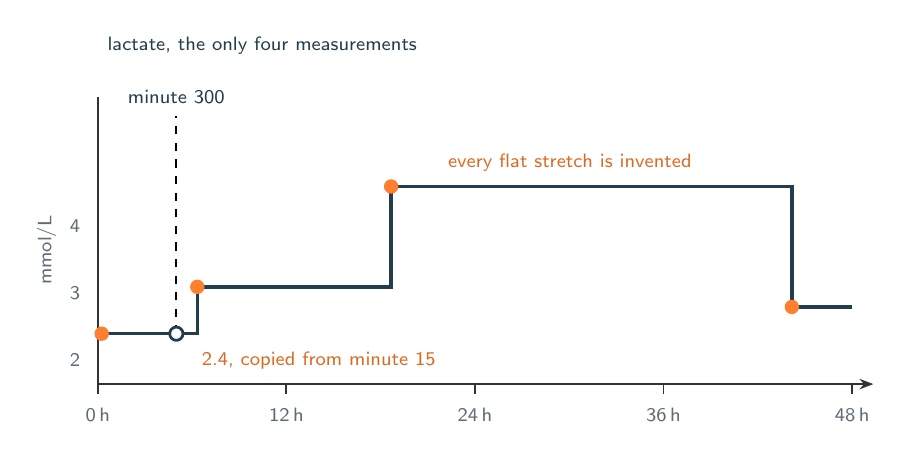
\begin{tikzpicture}[
    every node/.style={font=\sffamily},
    lab/.style={font=\sffamily\scriptsize, text=labelcolor},
    tag/.style={font=\sffamily\scriptsize, text=c2},
    hot/.style={font=\sffamily\scriptsize, text=c3!85!black},
]
\def\X#1{1.20 + #1*0.003333}
\def\Y#1{1.60 + (#1-2.0)*0.85}

\node[tag, anchor=west] at (1.20, 5.60) {lactate, the only four measurements};

\draw[axiscolor, line width=0.7pt] (1.20, 1.30) -- (1.20, 4.95);
\foreach \v in {2, 3, 4}{
    \node[lab, anchor=east] at (1.10, {\Y{\v}}) {\v};
}
\node[lab, rotate=90] at (0.55, 3.00) {mmol/L};

% the staircase written into the matrix
\draw[c2, line width=1.2pt]
    ({\X{15}}, {\Y{2.4}}) -- ({\X{380}}, {\Y{2.4}})
    -- ({\X{380}}, {\Y{3.1}}) -- ({\X{1120}}, {\Y{3.1}})
    -- ({\X{1120}}, {\Y{4.6}}) -- ({\X{2650}}, {\Y{4.6}})
    -- ({\X{2650}}, {\Y{2.8}}) -- ({\X{2880}}, {\Y{2.8}});

% the measurements themselves
\foreach \m/\v in {15/2.4, 380/3.1, 1120/4.6, 2650/2.8}{
    \fill[c3] ({\X{\m}}, {\Y{\v}}) circle (2.6pt);
}

% minute 300 sits on a flat
\draw[c1, line width=0.8pt, dashed] ({\X{300}}, {\Y{2.4}}) -- ({\X{300}}, 4.70);
\node[tag, anchor=south] at ({\X{300}}, 4.74) {minute 300};
\fill[white] ({\X{300}}, {\Y{2.4}}) circle (2.4pt);
\draw[c2, line width=1.0pt] ({\X{300}}, {\Y{2.4}}) circle (2.4pt);
\node[hot, anchor=west] at ({\X{300}+0.20}, {\Y{2.4}-0.34})
    {2.4, copied from minute 15};

\node[hot, anchor=west] at ({\X{1300}}, {\Y{4.6}+0.30})
    {every flat stretch is invented};

\draw[axiscolor, line width=0.8pt, -{Stealth[length=5pt]}] (1.20, 1.30) -- (11.05, 1.30);
\foreach \h in {0, 12, 24, 36, 48}{
    \pgfmathsetmacro\m{\h*60}
    \draw[axiscolor, line width=0.7pt] ({\X{\m}}, 1.30) -- ({\X{\m}}, 1.18);
    \node[lab, anchor=north] at ({\X{\m}}, 1.12) {\h\,h};
}
\end{tikzpicture}
\end{document}
